% Research continuation notes; intended for integration into the parent article.
% Requires amsmath, amssymb, amsthm, and the usual theorem environments.

\section{The singular elementary endpoint of the Lerch deformation}
\label{lerchboundary:sec:zero}

The large-derivative theorem in the zero-geometry chapter of the pinned manuscript
gives exactly $n$ simple positive zeros once $k$ is sufficiently large,
uniformly for $0\leq\rho\leq1$.  The following result describes a different
limit: $n$ and $k$ are fixed and the Lerch parameter tends to its elementary
endpoint $\rho=0$.  A multiple elementary zero generally sends most of its
branches off the real axis.  Consequently neither saturation nor the
one-index monotonicity theorem extends indiscriminately to higher indices.

Use the notation of Section~\ref{lerchboundary:sec:background} and introduce the
normalization
normalization
\begin{equation}\label{lerchboundary:eq:G}
 G_{n,k}(a,\rho)=\frac{(-1)^{n+k}}{k!}\mathcal D_{n,k}^{\rho}(a)
 =\sum_{m=0}^{\infty}\rho^m f_{n,k}(a+m),\qquad
 f_{n,k}(u)=\frac{P_{n,k}(-\log u)}{u^{k+1}},
\end{equation}
where
\begin{equation}\label{lerchboundary:eq:P}
 P_{n,k}(x)=n![t^n]e^{xt}\prod_{j=1}^k(1+t/j)
 =\prod_{j=1}^k\left(1+\frac1j\frac{d}{dx}\right)x^n.
\end{equation}
The series in \eqref{lerchboundary:eq:G} is locally uniformly absolutely
convergent for $a>0$ and $0\leq\rho\leq1$, because $k\geq1$.
It also defines a jointly holomorphic function for $\Re a>0$ and
$|\rho|<1$, with the principal logarithm. The derivation of this exact
spectral representation is already in the manuscript; it is not a new
identity claimed here.

\begin{lemma}[Elementary roots and a common compact zero region]
\label{lerchboundary:lem:roots}
Fix integers $n\geq1$ and $k\geq1$.
If $n>k$, put $d=n-k$. Then $P_{n,k}$ has a zero of multiplicity exactly
$d$ at $x=0$ and $k$ distinct strictly negative zeros. If $n\leq k$, all
$n$ zeros are distinct and strictly negative.
There exist $0<\epsilon<A<\infty$, depending on $n,k$, such that every
positive zero of $G_{n,k}(\cdot,\rho)$, for every $\rho\in[0,1]$, lies
in $[\epsilon,A]$.
\end{lemma}

\begin{proof}
For a real-rooted polynomial $p$ and $c>0$, the zeros of $p+cp'$ away
from inherited multiple zeros solve
\[
 \frac{p'(x)}{p(x)}=-\frac1c.
\]
The left side is strictly decreasing between its poles.  There is one
new simple zero between consecutive distinct zeros of $p$ and one to
the left of the smallest zero.  An old root of multiplicity $r\geq2$
is inherited with multiplicity $r-1$; old simple roots are not inherited.
Starting from $x^n$ therefore gives the asserted root pattern through
the first $k<n$ operations.  At $k=n-1$ the zero at $0$ is simple; the
next operation makes every root strictly negative, and all subsequent
operations preserve simplicity and strict negativity.  The exact
coefficient at the inherited zero is
\begin{equation}\label{lerchboundary:eq:leading}
 P_{n,k}(x)=\frac{n!}{k!d!}x^d+O(x^{d+1})\qquad(n>k).
\end{equation}

Choose $A$ strictly larger than the largest positive zero of $f_{n,k}$.
For every $u\geq A$, $-\log u$ lies to the left of all the roots of the
monic polynomial $P_{n,k}$, so $f_{n,k}(u)$ has the fixed strict sign
$(-1)^n$.  Each summand in \eqref{lerchboundary:eq:G} has that sign
when $a\geq A$, including the nonzero $m=0$ term.

At the other endpoint, $f_{n,k}(a)\sim a^{-k-1}\log^n(1/a)\to+\infty$
as $a\downarrow0$.  For $0<a\leq1$, the tail has a uniform absolute bound
\[
 \sum_{m=1}^{\infty}\rho^m|f_{n,k}(a+m)|
 \leq C_{n,k}\sum_{m=1}^{\infty}
       \frac{1+\log^n(m+1)}{m^{k+1}}<\infty.
\]
Consequently $G_{n,k}(a,\rho)>0$ for all sufficiently small positive
$a$, uniformly for $\rho\in[0,1]$.  This proves the common compact
zero region; in particular, no unobserved real zeros can escape to
$0$ or infinity in the parameter limits below.
\end{proof}

\begin{theorem}[Complete small-$\rho$ classification]
\label{lerchboundary:thm:smallrho}
Fix integers $n>k\geq1$ and put $d=n-k$ and
\begin{equation}\label{lerchboundary:eq:Delta}
 \Delta_{n,k}=
 \frac{(-1)^d k!d!}{2^{k+1}n!}P_{n,k}(-\log2).
\end{equation}
Then $\Delta_{n,k}\neq0$.  For some $\rho_{n,k}>0$, and every
$0<\rho<\rho_{n,k}$, all positive zeros of
$G_{n,k}(\cdot,\rho)$ are simple and their exact number is
\begin{equation}\label{lerchboundary:eq:count}
 N_{n,k}(\rho)=
 \begin{cases}
 k+1,&d\text{ odd},\\
 k+2,&d\text{ even and }\Delta_{n,k}<0,\\
 k,&d\text{ even and }\Delta_{n,k}>0.
 \end{cases}
\end{equation}
Here the number is both the number of distinct positive zeros and the
number counted with multiplicity, because simplicity is part of the
conclusion.

More precisely, the $k$ zeros corresponding to the nonzero elementary
polynomial roots extend as real analytic simple branches in $\rho$.
All $d$ complex zero branches issuing from $a=1$ have convergent Puiseux
expansions
\begin{equation}\label{lerchboundary:eq:puiseux}
 a_\nu(\rho)=1+z_\nu\rho^{1/d}+O_{n,k}(\rho^{2/d}),
 \qquad z_\nu^d=-\Delta_{n,k},\quad 1\leq\nu\leq d.
\end{equation}
The error describes fixed $n,k$; no uniformity as the two integer indices
vary is asserted.  If $n\leq k$, the elementary endpoint already has
$n$ simple zeros and exactly $n$ simple positive zeros persist for all
sufficiently small nonnegative $\rho$.
\end{theorem}

\begin{proof}
The polynomial $P_{n,k}$ is nonzero and has rational coefficients.
The classical Hermite--Lindemann theorem implies that $\log2$ is
transcendental: a nonzero algebraic logarithm would have transcendental
exponential, whereas $\exp(\log2)=2$. Hence
$P_{n,k}(-\log2)\neq0$.  Only this nonvanishing consequence of classical
transcendence theory is needed here; its source is Lindemann \cite{Lindemann1882}.

Put $\delta=a-1$.  Joint analyticity near $(a,\rho)=(1,0)$ and
\eqref{lerchboundary:eq:leading} give
\begin{equation}\label{lerchboundary:eq:local}
 G_{n,k}(1+\delta,\rho)
   =\delta^d A(\delta)+\rho B(\delta,\rho),\qquad
 A(0)=\frac{(-1)^d n!}{k!d!},\quad
 B(0,0)=\frac{P_{n,k}(-\log2)}{2^{k+1}}.
\end{equation}
Set $\rho=s^d$. The function
\[
 H(z,s)=z^d A(sz)+B(sz,s^d)
\]
is holomorphic near every point $(z,0)$ with $z$ bounded, and
$H(z,0)=A(0)(z^d+\Delta_{n,k})$ has exactly $d$ distinct roots.
The holomorphic implicit function theorem gives a convergent power
series $z_\nu(s)$ through each of them. Thus
$a_\nu=1+s z_\nu(s)$ proves \eqref{lerchboundary:eq:puiseux}.
Choose a fixed small complex disk about $a=1$ containing no other
zero of $G_{n,k}(\cdot,0)$.  Uniform convergence on its boundary and
Rouche's theorem show that it contains exactly $d$ zeros, with
multiplicity, for all sufficiently small $\rho$.  The $d$ branches
just constructed account for all of them.

For real positive $s$, the branches through real $z_\nu$ remain real
by uniqueness and complex conjugation, and the branches through
nonreal $z_\nu$ remain nonreal by continuity. Every branch is simple,
since $H_z(z_\nu(s),s)\neq0$ for sufficiently small $s$.  An odd-degree
equation $z^d=-\Delta_{n,k}$ has exactly one real root. An even-degree
equation has two real roots if $\Delta_{n,k}<0$ and none if
$\Delta_{n,k}>0$.  These real branches have positive $a$ for small $s$.

The other $k$ elementary zeros are simple and positive, so ordinary
implicit continuation supplies exactly one real simple zero in each
of $k$ disjoint small disks about them.  On the complement of these
disks and the disk about $1$ in the compact real interval supplied
by Lemma~\ref{lerchboundary:lem:roots}, the continuous function
$G_{n,k}(\cdot,0)$ is bounded away from zero.  Locally uniform
convergence excludes additional real zeros there.  This proves
\eqref{lerchboundary:eq:count} globally, not merely near the elementary
zeros.  If $n\leq k$, the same argument with only simple-root disks
proves the last assertion.
\end{proof}

The sign of $\Delta_{n,k}$ is effective for any specified $(n,k)$:
interval Horner evaluation of a rational polynomial at rational
enclosures for $\log2$ eventually separates it from zero.  The
nonvanishing theorem proves termination.  The theorem does not give
an explicit numerical value of $\rho_{n,k}$; such a value would require
quantitative versions of the compact and local perturbation estimates.

\begin{corollary}[First derivative: one or two zeros near the elementary endpoint]
\label{lerchboundary:cor:k1}
For every fixed $n\geq2$, $\mathcal D_{n,1}^{\rho}$ has exactly one
simple positive zero for all sufficiently small $\rho>0$ if $n$ is
odd, and exactly two if $n$ is even.  One zero is a real analytic
perturbation of $e^n$.  If $n$ is even, the second is
\begin{equation}\label{lerchboundary:eq:k1small}
 a_{\mathrm{small}}(\rho)
 =1-\log2\left(\frac{n-\log2}{4n}\right)^{1/(n-1)}
      \rho^{1/(n-1)}+O_n(\rho^{2/(n-1)}).
\end{equation}
\end{corollary}

\begin{proof}
Here $P_{n,1}(x)=x^{n-1}(x+n)$, so
\[
 \Delta_{n,1}=
   \frac{(\log2)^{n-1}(n-\log2)}{4n}>0.
\]
Apply Theorem~\ref{lerchboundary:thm:smallrho}, noting that the unique
nonzero elementary root is $x=-n$ and hence $a=e^n$.
\end{proof}

\begin{corollary}[Interior degeneracy is forced at indices three and four]
\label{lerchboundary:cor:degeneracy}
For each $n\in\{3,4\}$ there exist $0<\rho_*<1$ and $a_*>0$ such that
\[
 \mathcal D_{n,1}^{\rho_*}(a_*)=0,
 \qquad \partial_a\mathcal D_{n,1}^{\rho_*}(a_*)=0.
\]
\end{corollary}

\begin{proof}
The manuscript's proved $\rho=1$, $k=1$ certificates give $n$ simple
positive zeros.  They persist for $\rho<1$ sufficiently close to $1$:
locally uniform convergence in both the function and its $a$-derivative
gives a sign change and a nonzero derivative in a neighborhood of each
old zero. The global bound of at most $n$ zeros with multiplicity then
gives exactly these $n$ zeros.
Corollary~\ref{lerchboundary:cor:k1} gives respectively one and two
zeros near $\rho=0$. If every positive zero for $0<\rho<1$ were simple,
the implicit function theorem and the common compact zero region would
make the number locally constant throughout the connected interval
$(0,1)$. This contradicts the two endpoint counts.
\end{proof}

This proves the existence of a multiple-zero event.  It does not prove
that an event is a unique nondegenerate saddle-node: assertions such as
$\partial_a^2G(a_*,\rho_*)\neq0$ and
$\partial_\rho G(a_*,\rho_*)\neq0$ require additional analysis.

\section{A rigorous obstruction to monotonicity of higher zero branches}
\label{lerchboundary:sec:monotonicity}

\begin{proposition}[Sensitivity of an elementary simple zero]
\label{lerchboundary:prop:sensitivity}
If $r>0$ is a simple zero of $f_{n,k}$ and $a(\rho)$ is its analytic
continuation as a zero of $G_{n,k}$, then
\begin{equation}\label{lerchboundary:eq:sensitivity}
 a'(0)=-\frac{f_{n,k}(r+1)}{f'_{n,k}(r)}.
\end{equation}
\end{proposition}

\begin{proof}
Differentiate $G_{n,k}(a(\rho),\rho)=0$ at $\rho=0$ in the normally
convergent series \eqref{lerchboundary:eq:G}.
\end{proof}

\begin{theorem}[The smallest zero can move to the right]
\label{lerchboundary:thm:counterexample}
There exists $\rho_0>0$ such that $\mathcal D_{4,3}^{\rho}$ has exactly
four simple positive zeros for $0\leq\rho<\rho_0$. Its smallest zero
$a_1(\rho)$ satisfies $a_1(0)=1$ and
\begin{equation}\label{lerchboundary:eq:counterexample}
 a_1'(0)=\frac{P_{4,3}(-\log2)}{64}>0,
 \qquad P_{4,3}(x)=x^4+\frac{22}{3}x^3+12x^2+4x.
\end{equation}
In particular, the statement that every positive zero decreases with
$\rho$ is false, even when all zeros under consideration are simple
and the full allowed zero count is attained.
\end{theorem}

\begin{proof}
The polynomial has a simple zero at $0$ and three distinct negative
zeros by Lemma~\ref{lerchboundary:lem:roots}; hence the smallest
elementary positive zero is $1$. Its derivative in $a$ is
$f'_{4,3}(1)=-P'_{4,3}(0)=-4$ and
$f_{4,3}(2)=P_{4,3}(-\log2)/16$.
Equation~\eqref{lerchboundary:eq:sensitivity} gives the displayed value.

For an entirely rational sign proof put $L=\log2$.  The series
\[
 L=2\sum_{j=0}^{\infty}\frac{3^{-2j-1}}{2j+1}
\]
gives $2/3<L<3/4$. Therefore
\[
 L^3-\frac{22}{3}L^2+12L-4
 >\frac8{27}-\frac{22}{3}\frac9{16}+8-4
 =\frac{37}{216}>0.
\]
Since $P_{4,3}(-L)=L(L^3-\tfrac{22}{3}L^2+12L-4)$, its sign is
strictly positive.  Analytic continuation keeps the derivative
positive on a sufficiently small interval.  The root count and
ordering follow from Theorem~\ref{lerchboundary:thm:smallrho} with
$n=4,k=3,d=1$.
\end{proof}

The accompanying rational interval calculation sharpens the coefficient
to
\[
 0.0122109650329620<a_1'(0)<0.0122109650329621.
\]
The rigorous sign does not depend on these decimal enclosures.

\section{A full two-zero theorem and a nonmonotone branch}
\label{lerchboundary:sec:n2}

\begin{lemma}[A single change of coefficient sign]
\label{lerchboundary:lem:coefficient-sign}
Let $\sum_{m\geq0}|b_m|<\infty$. Suppose for an integer $M\geq0$ that
$b_m\leq0$ for $0\leq m\leq M$ and $b_m\geq0$ for $m>M$.
If $\sum_{m\geq0}b_m<0$, then
\[
 \sum_{m\geq0}b_m\rho^m<0\qquad(0<\rho\leq1).
\]
The same conclusion holds at $\rho=0$ if $b_0<0$.
\end{lemma}

\begin{proof}
For $0<\rho\leq1$, divide the absolutely convergent series by $\rho^M$.
For $m\leq M$, the inequality $\rho^{m-M}\geq1$ and $b_m\leq0$ give
$b_m\rho^{m-M}\leq b_m$. For $m>M$, the inequalities reverse for the
power but not for the final product: again
$b_m\rho^{m-M}\leq b_m$. Summing proves
\[
 \rho^{-M}\sum_{m\geq0}b_m\rho^m\leq\sum_{m\geq0}b_m<0.
\]
At $\rho=0$ the series equals $b_0$.
\end{proof}

\begin{theorem}[Two simple zeros throughout the deformation]
\label{lerchboundary:thm:n2global}
For every $\rho\in[0,1]$, the first parameter derivative
$\mathcal D_{2,1}^{\rho}$ has exactly two simple positive zeros
$a_1(\rho)<a_2(\rho)$, and
\begin{equation}\label{lerchboundary:eq:n2bracket}
 a_1(\rho)<\frac{13}{10}<a_2(\rho).
\end{equation}
Both branches are continuous on $[0,1]$ and real analytic on $[0,1)$.
The first branch is not monotone. More explicitly,
\begin{equation}\label{lerchboundary:eq:n2derivative}
 a_1(0)=1,\qquad
 a_1'(0)=-\frac{\log2(2-\log2)}8<0,
 \qquad a_1(1)>1.
\end{equation}
Consequently this branch has a minimum at some point of $(0,1)$.
\end{theorem}

\begin{proof}
The relevant elementary function is
\[
 f_{2,1}(u)=\frac{\log u(\log u-2)}{u^2}.
\]
At $a=13/10$, put $b_m=f_{2,1}(13/10+m)$.
These coefficients are negative while $13/10+m<e^2$ and positive
while $13/10+m>e^2$.  There is therefore a finite integer $M$ with
the coefficient pattern in Lemma~\ref{lerchboundary:lem:coefficient-sign}.
Moreover $b_0<0$, since $1<13/10<e^2$.  There is no need to determine
the numerical value of $M$.

The following exact rational enclosures come from the source's
zero-certificate appendix \cite{ProveItSnapshot}. The accompanying
verification script reproduces them:
\begin{align}
 G_{2,1}(1,1)&\in[0.11418372,\,0.11418373],
 \label{lerchboundary:eq:n2cert-one}\\
 (13/10)^2G_{2,1}(13/10,1)
 &\in[-0.12008911,\,-0.12008910].
 \label{lerchboundary:eq:n2cert-mid}
\end{align}
The positive normalization in the second line does not alter its sign.
Lemma~\ref{lerchboundary:lem:coefficient-sign} now gives
$G_{2,1}(13/10,\rho)<0$ for every $\rho\in[0,1]$.
By Lemma~\ref{lerchboundary:lem:roots} the sign is positive near
$a=0$ and for sufficiently large $a$, so there is a positive zero
on each side of $13/10$. The manuscript's global Laplace variation
bound is at most two zeros counted with multiplicity. Hence these
are exactly the two zeros and both are simple.

Simplicity gives analytic continuation locally in $\rho<1$, and the
fixed separating point $13/10$ preserves the branch ordering.
Uniform convergence and the common compact zero region give continuity
at $\rho=1$. The analytic statement at $0$ means that each branch has
a real analytic extension to a small interval about $0$.
At $\rho=0$ the smaller zero is $1$; either
\eqref{lerchboundary:eq:k1small} with $n=2$ or direct implicit
differentiation gives the derivative in \eqref{lerchboundary:eq:n2derivative}.
The signs \eqref{lerchboundary:eq:n2cert-one} and
\eqref{lerchboundary:eq:n2cert-mid} isolate a zero in $(1,13/10)$.
It must be $a_1(1)$ by the two-zero classification. Thus the branch
first decreases below $1$ and ultimately ends above $1$.  It is neither
nondecreasing nor nonincreasing. Its continuity on the compact interval
and these endpoint facts force its minimum into $(0,1)$.
\end{proof}

\begin{corollary}[The uniform saturation threshold at index two]
\label{lerchboundary:cor:n2allk}
For every $k\geq1$ and every $\rho\in[0,1]$,
$\mathcal D_{2,k}^{\rho}$ has exactly two simple positive zeros.
For fixed $\rho$, they strictly interlace to the right as $k$ increases.
Thus the smallest possible uniform saturation threshold at index two
is $K_2=1$.
\end{corollary}

\begin{proof}
Theorem~\ref{lerchboundary:thm:n2global} supplies saturation at $k=1$.
Apply the manuscript's persistence and rightward-interlacing theorem,
which follows from $F_{n,k+1}^{\rho}=-\partial_aF_{n,k}^{\rho}$ and the
global bound with multiplicity.
\end{proof}

The eleven rational endpoint signs replayed by the supporting script are
exactly the two signs above and the nine signs supplying the source
$n=3,4$ endpoint counts used in
Corollary~\ref{lerchboundary:cor:degeneracy}.  The underlying outward
integer Euler--Maclaurin routine is included verbatim, with its pinned
repository provenance recorded in the output data.

\begin{figure}[htbp]
\centering
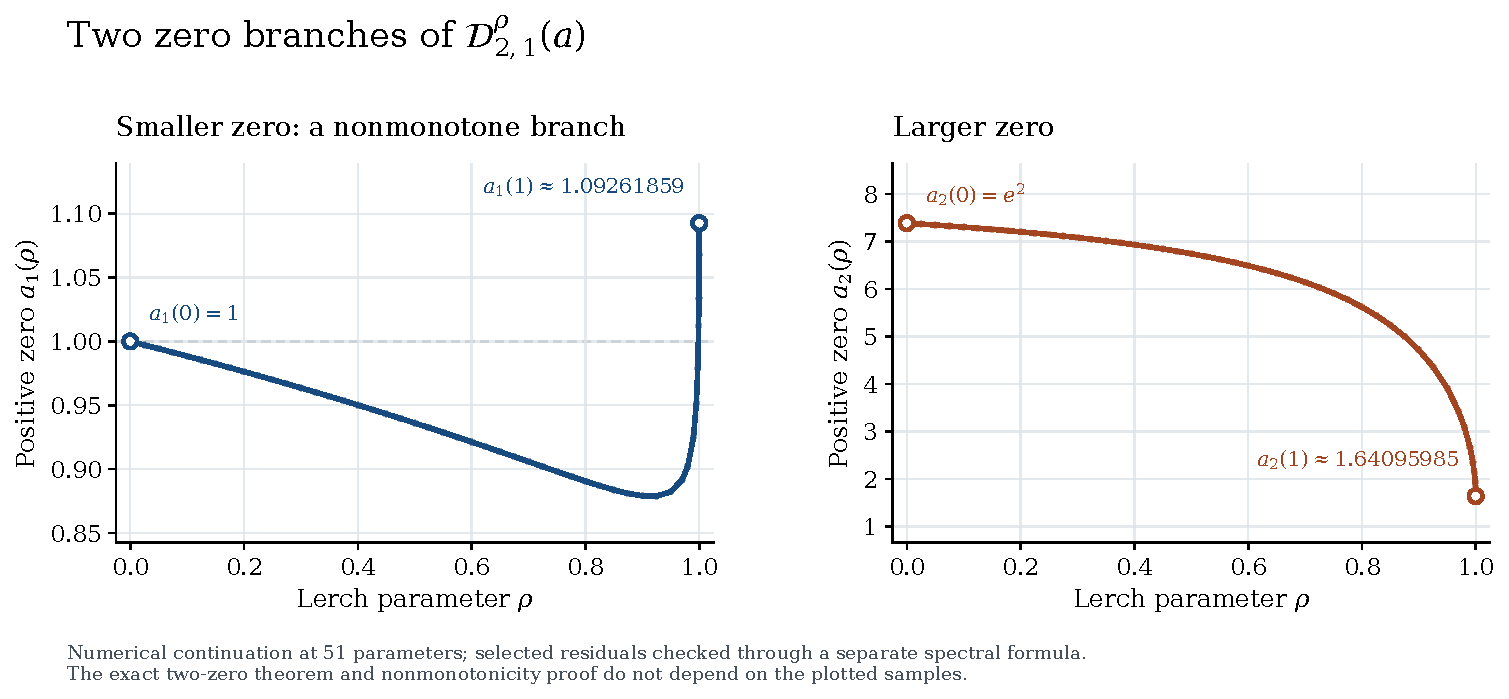
\includegraphics[width=\linewidth]{figures/lerch_n2_branches.pdf}
\caption{The two positive zeros of $\mathcal D_{2,1}^{\rho}(a)$,
computed at $51$ parameter values. The first branch is nonmonotone;
the second joins $e^2$ to approximately $1.6409598465$.
The curves and interior locations are numerical diagnostics. The
existence, simplicity, exact zero count, and nonmonotonicity of the
first branch follow independently from the proofs.}
\label{lerchboundary:fig:two-branches}
\end{figure}

The endpoint roots are numerically
$a_1(1)\approx1.0926185942922162563$ and
$a_2(1)\approx1.6409598465375973621$. Among the plotted samples, the
smallest first-branch value occurs at $\rho=0.925$, with
$a_1\approx0.878826386000143658$. This is a sampled minimum, not a
certified optimizer. The largest Laplace residual of the $102$ roots
is below $5.60\times10^{-30}$; $14$ independent Lerch/Hurwitz spectral
checks have residuals below $3.13\times10^{-30}$. Numerical rounding
is not interval-certified.

